\chapter{Birds-Eye View:\\Architecture and Use Cases}
In this chapter, we will take a birds-eye view at the architectures we wish to
implement with this thesis.
First, we will show how what architecture we need to
generate GPU kernels for \csharp{}, and then show a use case for such kernels.

Second, we show an architecture for making Futhark-generated GPU kernels from
\fsharp{} source code and using them in \fsharp{} projects, and then show a use
case for this architecture.

\section{Generating GPU accelerated libraries}
In this thesis, we are interested in making Futhark-generated GPU kernels available
in \csharp{} programs.
Currently, Futhark source code can be compiled to C and Python code.
For example, the Futhark C compiler follows the basic architecture shown in
figure \ref{fig:ccompiler}.
When we call the Futhark C compiler \texttt{futhark-c} on a Futhark source file, 
the compiler reads the source code file (and possibly imports) into a high-level
compiler representation.
As the compiler applies different passes to optimize the program, it also 
successively re-writes it using lower-level but still pure-functional 
intermediate representations (IR).  The last step in the blue box is to generate
an imperative IR, which is not subject to further Futhark optimizations.
This imperative IR is the input to various code generators, for example, 
the second box in the figure will perform a translation to the C language.
The resulting C souce file contains allows the exports of the original Futhark 
to be used in an intuitive fashion from any other C program.

The Python compilation pipeline follows a similar strategy.

\begin{figure}[H]
  \centering
  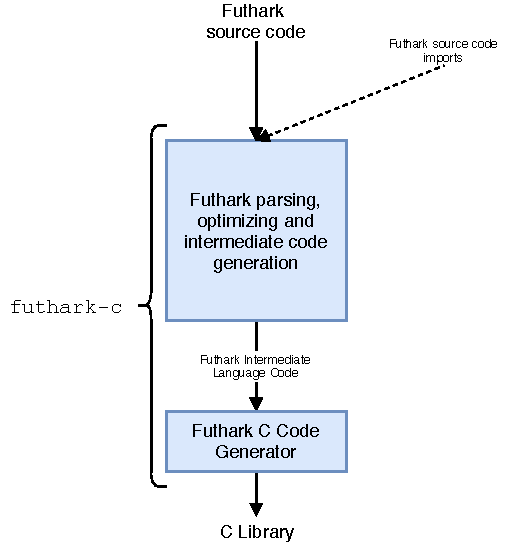
\includegraphics{chapters/figs/architecture/ccompiler.pdf}
  \caption{The Futhark-to-C compilation pipeline}
  \label{fig:ccompiler}
\end{figure}

\subsection{Using Futhark in Python}
We will now describe a use case for the Futhark-to-Python compiler:
\begin{enumerate}
\item We write a short Futhark program, which has a single entry function
    available. This program takes an array of integers, and
    adds 2 to each element in the array. The program is saved in file 
    {\tt mapPlus2.fut} and is shown below: %in figure \ref{fig:shortfutharkprogram0}.
\begin{lstlisting}[language=Futhark]
entry mapPlus2 (xs : []i32) : []i32 =
map (+2) xs
\end{lstlisting}

\item We then compile the Futhark program into a library file, by calling the
  Futhark compiler from the command line, as shown below: %in figure \ref{fig:shortfutharkprogram1}.
  \begin{lstlisting}[language=bash]
  $ futhark-py --library -o MapPlus2.py mapPlus2.fut
  \end{lstlisting}
  This compiles \texttt{mapPlus2.fut} to a Python file called {\tt MapPlus2.py}.
  In essence, the transpilation process gathers all the Futhark entry-points into 
  a Python class, contained in a Python module, both named {\tt MapPlus2}.
  For example the Python class can be instantiated with different options,  
    which enable gathering profiling information, or, setting default values
    for program-parameters such as tile sizes of CUDA block sizes.

\item 
    Finally, we write a short Python program, which uses the exports (entry points) 
    of the original Futhark program, for example, the {\tt mapPlus2} function.
    One such simple program is shown below.
    \begin{minted}[linenos]{python}
  from MapPlus2 import MapPlus2

  def main():
    xs = range(1,1000000)
    mapPlus2Class = MapPlus2()
    xs2 = mapPlus2Class.mapPlus2(xs)
  \end{minted}
%Such a program is shown in figure \ref{fig:shortfutharkprogram2}.
  As expected, the Python program first imports the Futhark library on line 
    1 and then it constructs an instance of the corresponding class on line 5.\\
  On line 4, we generate an array of integers from 0 to 1000000, and finally
  on line 6, we use the Futhark function mapPlus2 to add 2 to every
  element in our array.
\end{enumerate}

%\begin{figure}
%\begin{lstlisting}[language=Futhark]
%entry mapPlus2 (xs : []i32) : []i32 =
%map (+2) xs
%\end{lstlisting}
%\caption{A short Futhark program called mapPlus2.fut}
%\label{fig:shortfutharkprogram0}
%\end{figure}

%  \begin{figure}
%\begin{lstlisting}[language=bash]
%  $ futhark-py --library -o MapPlus2.py mapPlus2.fut
%    \end{lstlisting}
%    \caption{We call the Futhark-to-Python compiler \texttt{futhark-py} on
%      mapPlus2.fut}
%    \label{fig:shortfutharkprogram1}
%  \end{figure}
  
%  \begin{figure}
%\begin{minted}[linenos]{python}
%  from MapPlus2 import MapPlus2
%
%  def main():
%    xs = range(1,1000000)
%    mapPlus2Class = MapPlus2()
%    xs2 = mapPlus2Class.mapPlus2(xs)
%  \end{minted}
%    \caption{We use the compiled Futhark program as any other library.}
%    \label{fig:shortfutharkprogram2}
%  \end{figure}
%\clearpage

\subsection{Using Futhark in \csharp{}}

The intended way for using Futhark-generated libraries from \csharp{}
follows faithfully the interface already used by Python (and C). 
For example a use case is described below: 

\begin{enumerate}
\item We write a short Futhark program, which has a single entry function
  available. This program takes an array of integers, and
adds 2 to each element in the array:
% The program is shown in figure \ref{fig:shortfutharkprogram3}. 
  \begin{lstlisting}[language=Futhark]
entry mapPlus2 (xs : []i32) : []i32 =
  map (+2) xs
  \end{lstlisting}


\item We then compile the Futhark program into a library file, by calling the
  Futhark compiler from the command line, %like shown in figure \ref{fig:shortfutharkprogram4}.
which will compile \texttt{mapPlus2.fut} to a \csharp{} file called MapPlus2.cs
  \begin{lstlisting}[language=sh]
$ futhark-cs --library -o MapPlus2.cs mapPlus2.fut
  \end{lstlisting}

\item Finally, we write a short \csharp{} program in which we want to integrate
  the {\tt mapPlus2} function in our program. Such a program is shown in 
    figure~\ref{fig:shortfutharkprogram5}.
  In this program, we are importing the Futhark library on line 2 and constructing
  an instance of the contained Futhark class on line 8.\\
  On line 9, we generate an array of integers from 0 to 1000000, and finally
  on line 10, we use the exposed Futhark function mapPlus2 to add 2 to every
  element in our array.
\end{enumerate}

%\begin{figure}[H]
%  \centering
%  \begin{lstlisting}[language=Futhark]
%entry mapPlus2 (xs : []i32) : []i32 =
%  map (+2) xs
%  \end{lstlisting}
%  \caption{A short Futhark program called mapPlus2.fut}
%  \label{fig:shortfutharkprogram3}
%\end{figure}
%
%\begin{figure}[H]
%  \centering
%  \begin{lstlisting}[language=sh]
%$ futhark-cs --library -o MapPlus2.cs mapPlus2.fut
%  \end{lstlisting}
%  \caption{We call the Futhark-to-\csharp{} compiler \texttt{futhark-cs} on
%    mapPlus2.fut}
%  \label{fig:shortfutharkprogram4}
%\end{figure}

\begin{figure}[H]
  \centering
\begin{minted}[linenos]{csharp}
using System.Linq;
using MapPlus2;

public class Program
{
    public static int Main(string[] args)
    {
        var mapplus2Class = new MapPlus2();
        var xs = Enumerable.Range(0, 1000000).ToArray();
        var xs_result = mapplus2Class.mapPlus2(xs)
    }
}
\end{minted}
  \caption{We use the compiled Futhark program as any other library.}
  \label{fig:shortfutharkprogram5}
\end{figure}

But to be able to achieve this, we must design and implement a Futhark \csharp{}
code generator.

\section{Transpiling \fsharp{} Computational Kernels to Futhark}
%\section{Obtaining and integrating GPU kernels from- and in high level
%  languages}

The second goal of this thesis is to create an architecture which allows the
user to express the computational kernels directly in a subset of a mainstream
language. (These kernels can be then integrated back into a mainstream 
program by means of the code generators discussed in the previous section.)
Specifically, we want to obtain GPU kernels directly from \fsharp{} source 
code, and to use these kernels in a program written in \fsharp{} (or \csharp{}) 
afterwards.

In figure \ref{fig:fsharkcompiler}, we show such an architecture for the \fsharp{} language.

\begin{figure}[H]
  \centering
  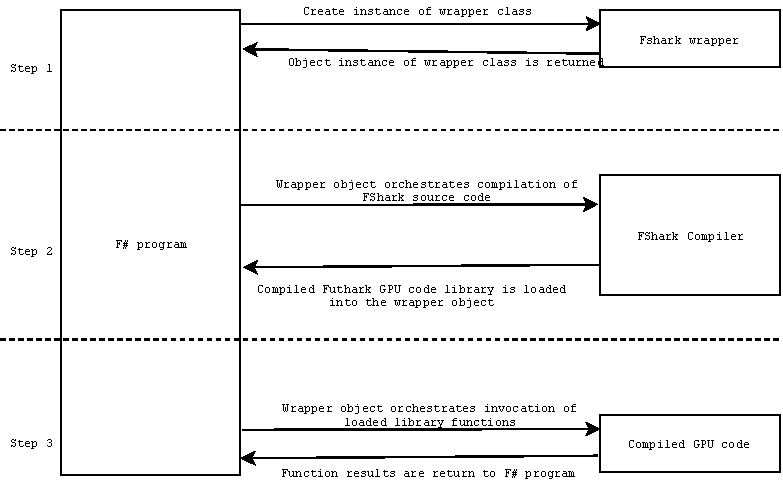
\includegraphics{chapters/figs/fsharkarchitecture.pdf}
  \caption{The \fshark{} architecture}
  \label{fig:fsharkcompiler}
\end{figure}

\subsection{A use case}
Following the architecture shown above, we demonstrate a use case which follows
the steps shown in the architecture.
\begin{enumerate}
\item  We write a small \fshark{} program that we wish to use in our \fsharp{}
  program to a file called \texttt{MapPlus2.fs}. Such an \fshark{} program is shown below:
\begin{minted}[linenos]{fsharp}
let saxpy (a : int) (x : int) (y : int) : int =
  a*x+y
  
[<FSharkEntry>]
let run_saxpy (a : int) (xs : int array) (ys : int array): int array =
  let res = Map2 (saxpy a) xs ys
  in res
\end{minted}

\item We create an instance of the \fshark{} wrapper class, add the file path
  of our \fshark{} program to it. Then we run the \fshark{} compilation to
  compile and load the \fshark{} program into the wrapper.
  This corresponds to step one and two in the architecture sketch, and is done
  in line 3-5 in figure \ref{fig:shortfsharkprogram1}.

\item Finally in line 7-10, we declare some arguments for our \fshark{} function, and pass
  them to the compiled \fshark{} program through the \fshark{} wrapper.
\end{enumerate}

\begin{figure}[h]
  \centering
\begin{minted}[linenos]{fsharp}
[<EntryPoint>]
let main =
  let fshark = new FShark()
  fshark.addSourceFile("MapPlus2.fs")
  fshark.CompileAndLoad()

  let a = 5
  let xs = Iota 10000
  let ys = Replicate 10000 1
  let res = fshark.InvokeFunction("run_saxpy", a, xs, ys)
\end{minted}
  \caption{Compiling and using MapPlus2.fs from within an \fsharp{} program.}
  \label{fig:shortfsharkprogram1}
\end{figure}



%%% Local Variables:
%%% mode: latex
%%% TeX-master: "../thesis"
%%% End:
